\documentclass[10pt,twocolumn]{article}

\usepackage{times}
\usepackage{fullpage}

\usepackage{booktabs}  % for \midrule
%\usepackage{subfigure}
\usepackage{balance}
\usepackage{graphicx}
\usepackage{xspace}
%\usepackage{pslatex}
%\usepackage{pifont}
%\usepackage{multirow}
%\usepackage{array}
%\usepackage{booktabs}
%\usepackage{cite}
\usepackage{url}
%\usepackage{cancel}
\usepackage{color,colortbl}
%\usepackage{microtype}
%\usepackage{textcomp}% http://ctan.org/pkg/textcomp
\usepackage{tabularx}
\usepackage{framed}
\usepackage[]{algorithm2e}
\SetAlFnt{\small}
\SetAlCapFnt{\small}
\usepackage{algorithmic}

\usepackage{listings}
%\usepackage{scrextend}
%\usepackage{mathtools}
\usepackage{pbox}

\let\labelindent\relax
\usepackage{enumitem}

%\usepackage{tikz}
%\usepackage{decorations.pathmorphing}
%\usepackage{assymb}

\usepackage[labelfont=bf]{caption}

%\theoremstyle{plain}
\newtheorem{theorem}{\bf{Theorem}}%[section]
\newtheorem{lemma}[theorem]{\bf{Lemma}}
\newtheorem{corollary}[theorem]{\bf{Corollary}}
\newtheorem{proofl}[theorem]{\bf{Proof}}
\newtheorem{proposition}[theorem]{\bf{Proposition}}

%\theoremstyle{definition}
\newtheorem{definition}{\bf{Definition}}%[section]
\newtheorem{observation}{\bf{Observation}}%[section] 

%\theoremstyle{remark}
\newtheorem{example}{\bf{Example}}
\newtheorem{notation}{\bf{Notation}}
\newtheorem{fact}{\bf{Fact}}

\usepackage{listings}
\lstdefinelanguage{cs}
{
  morekeywords={abstract,event,new,struct,as,explicit,null,switch
		base,extern,this,bool,false,operator,throw,
		break,finally,out,true,byte,fixed,override,try,
		case,float,params,typeof,catch,for,private,uint,
		char,foreach,protected,ulong,checked,goto,public,unchecked,
		class,if,readonly,unsafe,const,implicit,ref,ushort,
		continue,in,return,using,decimal,int,sbyte,virtual,
		default,interface,sealed,volatile,delegate,internal,short,void,
		do,is,sizeof,while,double,lock,stackalloc,
		else,long,static,enum,namespace,string,
		where, from, select, group,by, having, into, many,
		every,
                function,
		or, and, on, var, when,let, zip, combine,
		minute,hour,day,week,year,calendar,count, Delay, Until, TakeUntil, Sample, Skip, Throttle},
	  sensitive=true,
	  morecomment=[l]{//},
	  morecomment=[s]{/*}{*/},
	  morestring=[b]",
}

\lstset{
	language=cs,
	tabsize=2,
        basicstyle=\small,
%        basicstyle=\normalsize,
        %upquote=true,
%        aboveskip={1.5\baselineskip},
        columns=fullflexible, %fixed,
        showstringspaces=false,
        extendedchars=true,
        breaklines=true,
%      prebreak = \raisebox{0ex}[0ex][0ex]{\ensuremath{\hookleftarrow}},
%	frame=single,
        showtabs=false,
        showspaces=false,
       identifierstyle=\ttfamily,
        keywordstyle=\color[rgb]{0,0,.8},% \sffamily,
        commentstyle=\color[rgb]{0.133,0.445,0.133},
%        stringstyle=\color[rgb]{0.627,0.126,0.941},
	numbers=left,
	xleftmargin=17pt,
%	tabsize=2
	captionpos=b,
	breakatwhitespace=true,     % sets if automatic breaks should only happen at whitespace
}

\newcommand\mypara[1]{\vspace{.3em}\noindent\textbf{#1}}
\newcommand{\urlwofont}[1]{\urlstyle{same}\url{#1}}

\newcommand{\dinv}{Dinv\xspace}
\newcommand{\scc}{strongly consistent cut\xspace}

%%%%%%%%%%%%%%%%%%%%%%%%%%%%%%%%%%%%%%%%
% Useful reviewing/feedback annotations
\usepackage{ifthen}
\usepackage[normalem]{ulem} % for \sout
\usepackage{xcolor}
\usepackage{amssymb}

\newcommand{\ra}{$\rightarrow$}
\newboolean{showedits}
\setboolean{showedits}{true} % toggle to show or hide edits
\ifthenelse{\boolean{showedits}}
{
	\newcommand{\ugh}[1]{\textcolor{red}{\uwave{#1}}} % please rephrase
	\newcommand{\ins}[1]{\textcolor{blue}{\uline{#1}}} % please insert
	\newcommand{\del}[1]{\textcolor{red}{\sout{#1}}} % please delete
	\newcommand{\chg}[2]{\textcolor{red}{\sout{#1}}{\ra}\textcolor{blue}{\uline{#2}}} % please change
}{
	\newcommand{\ugh}[1]{#1} % please rephrase
	\newcommand{\ins}[1]{#1} % please insert
	\newcommand{\del}[1]{} % please delete
	\newcommand{\chg}[2]{#2}
}

\newboolean{showcomments}
\setboolean{showcomments}{true}
%\setboolean{showcomments}{false}
\newcommand{\id}[1]{$-$Id: scgPaper.tex 32478 2010-04-29 09:11:32Z oscar $-$}
\newcommand{\yellowbox}[1]{\fcolorbox{gray}{yellow}{\bfseries\sffamily\scriptsize#1}}
\newcommand{\triangles}[1]{{\sf\small$\blacktriangleright$\textit{#1}$\blacktriangleleft$}}
\ifthenelse{\boolean{showcomments}}
%{\newcommand{\nb}[2]{{\yellowbox{#1}\triangles{#2}}}
{\newcommand{\nbc}[3]{
 {\colorbox{#3}{\bfseries\sffamily\scriptsize\textcolor{white}{#1}}}
 {\textcolor{#3}{\sf\small$\blacktriangleright$\textit{#2}$\blacktriangleleft$}}}
 \newcommand{\version}{\emph{\scriptsize\id}}}
{\newcommand{\nbc}[3]{}
 \renewcommand{\ugh}[1]{#1} % please rephrase
 \renewcommand{\ins}[1]{#1} % please insert
 \renewcommand{\del}[1]{} % please delete
 \renewcommand{\chg}[2]{#2} % please change
 \newcommand{\version}{}}
\newcommand{\nb}[2]{\nbc{#1}{#2}{orange}}

\definecolor{ibcolor}{rgb}{0.4,0.6,0.2}
\newcommand\iv[1]{\nbc{IB}{#1}{ibcolor}}
\usepackage{wasysym}
\newcommand\yesml[1]{\nbc{ML {\textcolor{yellow}\sun}}{#1}{mircolor}}

\definecolor{sgcolor}{rgb}{0.2,0.0,0.5}
\newcommand\sg[1]{\nbc{SG}{#1}{sgcolor}}

\definecolor{samcolor}{rgb}{0.2,0.4,0.2}
\newcommand\sam[1]{\nbc{SC}{#1}{samcolor}}

\definecolor{hccolor}{rgb}{0.21,0.54,0.84}
\newcommand\hc[1]{\nbc{HC}{#1}{hccolor}}

% Todo Command
\definecolor{todocolor}{rgb}{0.9,0.1,0.1}
\newcommand{\todo}[1]{\nbc{TODO}{#1}{todocolor}}


%%%%%%%%%%%%%%%%%%%%%%%%%%%%%%%%%%%%%%%%

\begin{document}

%\title{Inferring likely data invariants of distributed systems}
\title{Project Survey, fundemental distributed algorithms Inria 2017}
\author{Stewart Grant}
\date{}
\maketitle
%\thispagestyle{empty}

\section{Specification and verification of Dynamic Properties in Distributed Systems \\ \small\textit{Ozalp Babaoglu and Micheal Raynal ISIRA rennes}}

\subsection{Notes} interesting point early on that any number of events may be
"irrelevent with respect to a given property" so their model simply ignores
all that are not relevent. In the future consider providing a feild or
annotation in a messaging block, (such as govector) which would allow the
isolation of messages which pertained to a given property. This would allow
for a higher degeree of fidelity. In addition it may be possible to associate
messages with a given functionality based on their structure.

\noindent\textbf{run} a total order of events in a distributed system. This is what really hapend, but is unobservable due to clock skew, and an absent centralized clock.

Exampes of predicates which cannot be satisfied by a simple boolean predicate $A \vee B \wedge C$ where $A$, $B$, $C$ are variables.

\begin{itemize}
    \item Load ain the network is blaances.
    \item Resource allocation violates the \"at most k-out-of -n\" concurrent access requirement
    \item Message delay alone the route for A to B is less than 5ms
    \item No more than 100 total users logged in to tmachines A, B, and C
    \item In the computation of Fig 1 $x >= 2y$.
\end{itemize}

\noindent\textbf{sequence spec is an ordered array of simple predicates $SS ::= SP | SS; SP$}

Interval controlled sequences are a key component to realizing temporal
predicates esentially the process is as follows. An obervation is a set of
states $\Sigma$ on which a property can hold. A mentioned in the prior section
$SS ::= SP | SS; SP$ is a sequence of simple properties which hold over subsets
of an observation. Temporal properties can be constructed by linking
predicates. In the form $\phi;[\bar{\Theta}];\phi$ where all such phi are
observations on which a predicate holds.

$\phi_1;[\theta];\phi$ is satisfied by an observation if there exists a global
state $\Sigma^1$ in which $\phi_1$ holds, a late global state $\Sigma^2$ in
which $\phi_2$ holds, and $\Theta$ does not hold in the global states in
between. Denoted in the form $\phi_1;[\bar{\Theta}]\phi_2$.

This paper makes the contribution of formualting temporal strings of if
\textit{interval-constraied sequest} with the synyax
$\bar{[\Theta_1]}\phi_1;\dots;\bar{[\Theta_m]}\phi_m;\bar{[\Theta_{m+1}]}$

Key takeaway from the formulation. The difference between SS and ICS is that
between states $i_n,i_{n+1}$ there exists a $\bar{[\theta_n]}$ which must not
hold on that interval. In that way the expressivness of ICS is greater than
that of SS.

Two algorithms are proposed for solving SS \textbf{Pos} and \textbf{Def}. To
compute Def all paths through an observation are taken and must show that the
$SS$ formula holds. In constrast $SS$ \textbf{Pos} is verified simply by
finding a single example in an observation on which the formula holds.

\subsection{Take Away}

This paper presented a novel formulation for describing temporal properties in
distributed executions. It is very similar to \dinv in that it uses a latice to
formulate an execution. However, where \dinv prunes the search space by
examining only strongly consistant cuts, this approach dives in deeper, and
actually traverses all possible interleavings in order to satisfy a predicate.

If \dinv were to take this approach it would require that a user specify their
invariants ahead of time, if not then all possible observations of a run would
need to be fed into Daikon.

Of specific interest is their formulation of $\bar{[\theta]}\phi$ in that it
requirs some invariant to not hold before a know property in a given state.
Using \dinv's ground states this same technique could still be applied,
although it would be equally restricted by ground states. However, this could
still be a potential extension.

The clear problem with mining invariants using this technique is that it is a
search, therfore any attempt to infer invariants would result in inferring on
the entire search space.

This approach does not take into account failures, it could also be interesting
to extend the expressivness of the formula to accept failures and restarts. The
hardest part in this would be modifing $\Sigma$ to accept "Global" predicates
on a subset of nodes. Further it would be interesting to see if predicates
could be defined which allows for the recovery of a node, by a new one
introduced to the system.

Overall this is just a scheme for temporal logic detection in a system
instrumentd with vector clocks. It could be used for that golden key value spec
$\forall get(x) \leftarrow put(x) get(x) == get(x)$ untill $put(x')$. This would have been a cool path to go down if it had not allready been done.

\subsection{Questions}

\begin{itemize}
    \item Is there a way to divide temporal search paths for mining?
    \item Is there a way to identifiy identical search paths and merge them for compression?
       \item Is there an obvious or non obvious way to trim a search path, or limit the lenght of a search for temporal invariant mining?
       \item Can Search Paths be presented to daikon in a way which preserves temporal logic?
\end{itemize}





\section{On the Fly Testing of Regular Patterns in Distributed Computations \\
\small{Eddy Fromentin, Michel Raynal Vijay k Garg, Alex Tomlinson}}

\subsection{Notes}

This work aim to detect regular patterns in the exectuion of distrubted
systems. The first technique to note is that they reduced a distributed
execution down to only events corresponding to msg receves and sends. This is
the same intuition I had when initially building GoVector, and insturmenting
systems for \dinv but it is done formally.

Their technique relies on labling events with a symbol in an execution
language. Series of events form automata which are describable by regualr
expressions. Not sure where this paper is going, but I assume that they are
going to describe a partially orded regex syntax.

This paper did not go much further, the algorithm for performing on the fly
regular expressions is relativly simple. Essentally every process maintains an
array of the regular expression. The expression nessisarily begins at the
beginning of the computation, with omits much of the complexity incurred in the
\textit{specification and verification of dynamic properties in distributed
computation} paper. Each process maintains a boolean array of the properties in
the regex. When a new event occurs locally the process checks if it violates
the regex. Otherwise two seperate cases occur. 1) a sent message is received or
a local event happens, merge the two and check if they violate any of the regex
conditions. On a send event just treat it as a local event. In addition to
vector clocks the array of regular experession must be added to messages.

\subsection{Observations}

I think that regular expressions on states are interesting, but ultimatly not
going to play into my work. These models could be usefull for specifing
something like TCP where the execution is known to be finite, or should be. In
typical system cases though I believe that specifications need to be more
expressive than regular expersions. For instance Coq and TLA+ the key
languages in specification are fully fledged programming languages.

What this work does contribute is an online way to process regex. I think that
this is usefull for a couple of reasons 1) I think that it could be key in
generalizing some well known protocols such as leader election, where the set
of known messages would fit in the vocabulary of events.

I should do a bit of follow up on this work to see if anyone built a tool which
automatically translates regex into protocols rather than check a protocol with
regex, but I don't think that it would yeild interesting work.




\section{Shared Global states in Distrubted Computations \\ \small{Eddy
Fromentin, Michel Raynal}}

\subsection{Notes}

The paper begins with the same notation used in prior papers defining partial order and such. The key part of the paper is \textit{shared global states}, which are an element in the lattice of global states such that 

Let $\Sigma = (s_1,\dots,s_i,\dots,s_n) be a global state$ \\
$\Sigma is shared \iff $\\

$\forall (i,j)$ :: (prev($s_i$) $\rightarrow$ next($s_j$) \textit{or} $s_j =
s_j^{last} or s_i = s_i^0$)

Essentially a shared global state is a state which has the entire global
history as its transitive predisessor, or at least all of the history it could
known about transitivly.

The algorithm near the end of the paper shows how shared global state can be
detected on the fly, however the algorithm is centralized with diminishes how
interesting it is. That stated, shared global state is near conceptually with
common knowledge, in that it is the nth degree of eveyone knows everything, it
is the case that someone knows everything~\cite{Halpern:1990:KCK:79147.79161}.

\subsection{Observations}

While is is kind of cool that the idea of \textit{Shared Global States} has
been formalized here, there is a big want with reguard to purpose. Specifically
when would you want to use shared global state. I can only think of Chain
Replication.~\cite{vanRenesse:2004:CRS:1251254.1251261}. While shared global
state is not a central tenant of the system it would acheive it quite often
during execution.

With reguard to Dinv this is almost certanly not the path to go down, SCC are
allready too much of a restriction as they do no even consider the world of
\textit{observations}. With that said GSS could be an interestin root at which
to perform some sort of analysis. It serves as an obvious break point.

If I wanted to infer arbetrary temporal properties on a distributed execution I
could for instance make users provide a template, search for observations from
GSS roots, enumerate them in a key value store, overlay matching or equivalent
states (there would be few, but some may match the template.

This is probably not the way to go either, the size of the output would be
gigantic, just note that \textbf{GSS can be used for roots of computation} as
they are as close to common knowledge as you are ever going to get (and it can
be done on the fly)

\subsection{Questions}

\begin{itemize}

\item Is shared global state sufficient to coordinate locks? If not what
information is required to allow for locking?

\item How frequently do these happen in practice, for example in etcd? If the
answer is kind of frequently there may be some interesting work to be done.

\end{itemize}





\section{On-the-fly analysis of distributed computations \\
\small{Eddy Fromentin, Claude Jard, Guy-Vincent Jourdan, Michel Raynal}}

\subsection{Overview}

This paper proposed a method for checking properties of distributed
computations during exectuon. The Idea is a bit suble, and very general. Given
a standard model of a distrubuted systems ie $P_0 \dots P_n$ processand with
events $e_0 \dots e_m$ apply to each event a work or subset of an alphabet
$\Sigma$. As control flow passes through events on different machines check the
current alphabet againts a specified automata or regular expression. If an
event fails to correlate with the regular expression then it has not met the
specification and fails. Otherwize the letters of the event are appended to the
message, and upon the next event it is checked againts the regex again.

There is a little bit in the beginning about simplifing a distributed execution
down to an LPO. The graph (Figure 1b) does not make a lot of sense. It seems to
trim out long messages, and only be concerned with the longest message path
through the execution. It was not totally clear to me why this would be used,
but I guess the idea is that newer messages have some sort of precident, and
can invalidate old messages??



\section{Efficient Distributed Detection of Conjunctions of Local Predicates \\ \small{ Michel Hurfin, Masaaki Mizuno, Michel Raynal, Mukesh Sighal}}

\subsection{Notes}

The collapastion of internal events, ie the job done by the key-value store in
\dinv is refered to here as an interval. More precisely "the \textit{x}'th
interval of proces $P_i$ denoted by $\theta_i^x$ is a segment of the
computation that begins at event $e^x_i$ and ends at $e^{x+1}_i$. This
definiation may be usefull in describing the usage of the key value store, and
this citation, along with \todo{\textit{on the fly analysis} \& \textit{shared
global state} and others $\dots$ would be usefull. Thanks Raynal}

In early \dinv I defined a total ordering on cuts. Although I never ended up
using it becuase it was too course grain the same dependency is defined here.
Formally: A dependency relation denoted by $\rightsquigarrow$ is defined over
the set of all consistent cuts as follows. Let 

$C^x$ = $\theta^{x_1}_1, \theta^{x_2}_2, \dots , \theta^{x_p}_p$ 
and 
$C^y$ = $\theta^{y_1}_1, \theta^{y_2}_2, \dots , \theta^{y_p}_p$ 
be two consistent cuts, then: 
$C^x \rightsquigarrow C^y \iff (C^x \neq C^y) \wedge (\forall k, 1 \leq k \leq p , x_k \leq y_k)$ 

This algorithm is very technical, but somewhat similar to \dinv. Essentailly it
aims to show that at some point in relative time a conjunction of local
predicates held. The algorithm involves two vector clocks and a boolean vector
denoting predicate satisfiability of on a process. 

I think the algorithm goes like this.  If a predicate is true, set $P_i$ to
true. If you get a message with $P_j$ = true update the predicate array. Mark
the current vector time, and keep track of the first point in time the
predicate was denoted true. If $\theta$ becomes false set all incomming and
outgoing predicate messages to false. The predicate becomes true if there is a
causal path across all processes such that $\forall i \theta_i = true$. It is
not super complicated, the hard part is really just that it is done on the fly.

I think that this algorithm is a bit pessamistic, using a lattice I think that
these predicates could be detected more easily.

\subsection{Observations} 

This work is very specific. It aims to detect global predicates online, with
significant computational overhead. I think that the key takeaway from the
algorithm is the technique for detecting causal intervals online. Essentially
taint tracking and merging across multiple processes to show that some property
$\theta$ is satsified globally.

This work seeks to show that a given predicate is recognized globally and does not have any interaction with a state machine. Could this online technique be used as an atom to verify sequences in in computation, and allow for decentralized distributed computation? For instance would it be possible to encode a bunch of tasks, and have a single process issues a continue message once the task is complete? If the satisfaction of a given task is monotonic then I believe that the answer is yes.

\subsection{Questions}

\begin{itemize}

    \item Could this technique be used to easily distribute SAT solving? my
inital instinct is no, because there is no obvious way to do back propagation.

    \item Is this applied anywhere? For instance this could be used to show
something like termination in Hadoop withought a specified leader. With that
stated it would be a bit of overkill.

    \item could this be used to simplify termination in graph processing? Is
this this a more robust solution to predicate dection than the
\textit{White/Black} graph coloring that pregal uses.

    \item Is there a recovery mechanism for satisfied predicates? It seems like
in the worst case only a single process will learn that the predicate is
satisfied.

\end{itemize}

\section{Detecting Atomic Sequences of Predicates in Distributed Computations, 1993 \\ 
\small{Hichel Hurfin, Noel Plouzeau, Micheal Raynal}}

\subsection{Notes}

The goal of this paper is to detect sequences of atomic properties. I assume
that these would be something similar to the detection of distributed mutual
exclusion. The key inisght that was presented in the abstract is that these
properties on not monotonic. Perhaps this means that atomic properties may hold
on the \textbf{POS} predicate? I'm not sure because for the sake of guarentted
atomicity \textbf{DEF} seems to be a nessisary constraint.

Key note, the definition of "Atomicity" in the case of this paper is a sequence
of events, of which none violate a specific preperty ie $CA = \neg NP_1 \wedge
NP_2 \wedge \dots \wedge NP_n$. Where each $NP_i$ denots the property on a
select processes.

The real purpose of this paper is to count the number of causal paths which
satisfy a prefix of the form $do_0;[don't_0] do_1; [don't_1] \dots do_n$. This
differs from the specifing systems paper a little bit, essentially in the way
that they are counting the number of occurances.

\subsection{Observations}

An anti observation is, what is the purpose of this algorithm. It seems to be a
gneralization of the specification language, defined in Specification and
Verification of dynamic properties, but it is simply a counting function. I
suppose that the interesting bit comes from handing cases were predicates are
invalidated due to being non-atomic however, it was unclear to me why a counter
of these properties was wanted and not simply a flag.

This algorithm is extreamly clean. It would be interesting to see if it could
be extended to define a generalized decentralized computation framework similar
to Dryad but with a decentralized compute. Essentially all computations would
be defined as a set of predicates and antipredices, for instance, compute a
property on some large graph, and dont compute where any other node has.
Instances of conflict could be counted and reset. Individual functions could be
specified in this way, and entire programs could be written as a heirarchy of
predicates, and loops defined on them. Figuring out how to work in conditionals
would be a problem onto itself.

\subsection{Questions}

\begin{itemize}
    
    \item What common distributed debugging tasks actually require counts of invariant violations.

    \item Is it reasonable to define atomic predicates, with the execption of locking?

    \item Can this be leveraged in reverse, and turned into a control mechanism, rather than a checking algorithm.

\end{itemize}


\section{Some Optimal Algorithms for Decomposed Partially Ordered Sets \
\small{ Vijay K. Garag}}

\subsection{Notes}

I'm reading this one as both an introduction to Garag and as a bit of a break
from the proof heavy papers.

This paper allready seems like it is going to be a good resource, it has an
algorithm for detecting consistant cuts $n^2m$ time $\dots$ if this is really
the case, it may be possible just cut the crap on dinv and really speed it up.


As usual my hopes are dashed this is an early algorithm which only detects a
single consistant cut, not all of them like I had wanted. However, the online
variant may be useful for making \dinv a streaming service at some point.

The second algorithm in this paper checks if a set of given antichains compose
are constrained by a total ordering. The algorithm does so in $O(mn log n)$
time. Essentially it continuously merges sets of antichains untill it finds
aconflits where some set of antichains has events / elements $s$ and $t$ such
that $s || t $. It is a very nice algorithm, but given that \dinv never
encounters total orderings I don't think that it will come in handy.

\subsection{Observations}

The online detection of consistant cuts could be used as a fron end for dinv
easily, but the cost of checking all consistant cuts is still exponential.

\subsection{Questions}

\begin{itemize}

\item What is the purpose of finding largest antichains? Potentially it shows that the largest number of chains which can be composed is $n$ but it is still not clear where this would be applied. Is this to show the complexity during distributed debuggin?

\end{itemize}

\section{ Predicate Detection for Parallel Computation with Locking Constraints \\ \small{Yen-Jung Chang, Vijay K. Garag}}

\subsection{Notes}

Initially this paper proposes an analysis techinique which analyzes an
exponential number of posets in order to check if locking predicates hold. It
seems as if it is going to build posets out of code itself.

\textbf{After getting through the first 5 pages I was very lost. This paper it seems is too theoretical for me. \todo{Return to this paper after reading ~15 more theoretical papers by Garag}}

\section{Modeling, Analyzing and Slicing Periodic Distributed Computations \\ 
\small{Vijay K. Garag, Anurag Agarwal, Vinit Ogale}}

\subsection{Notes}

This paper proposes an anaylsis technique for decomposing distributed
exectutions. It proposes a very interesting model, in which DAG's are infinine.
Their proposed infanite DAG is reffered to as a \textit{d-diagram} and
essentially models looping computation post predicate on an infanite timeline.
They use this model to verify temporal properties such as liveness.

Not the useage of \textit{cut frontier}. This is proper usage and should be
intagrated into the \dinv paper if possible.

A very interesting addition on page 14 is the formalization of recursive vector
closk. It is simple algebra, but it states simply that given some initial
configuration $C$ lets say, and a continuing recursive computation, the vector
clock values for all events, of future computations can be computed a priori.

The paper continues by formulating how to verify liveness properties 

\subsection{Observations}

My immidate impression of this paper is that it falls short in its model of a
distributed execution. It only defines an infanite execution as a prefix
followed by a periodic set of recurrent transitions. It seems that this model
is strictly limited to a single periodic computation, and not a general
computation which must adapt to interaction.

For instance this model could be used to analyze a key value store which only
serverd puts, or gets, or a fininte repeatable sequence of accesses. It would
however fall short in the following scenarios.

I was interested in extending the model presented in this paper. As mentioned
in the prior paragraph there are a few shortcommings, such as the models
ability to only quantify a single infanite state. I drafted an extension to
this model on the board. 

\begin{figure}[t]
    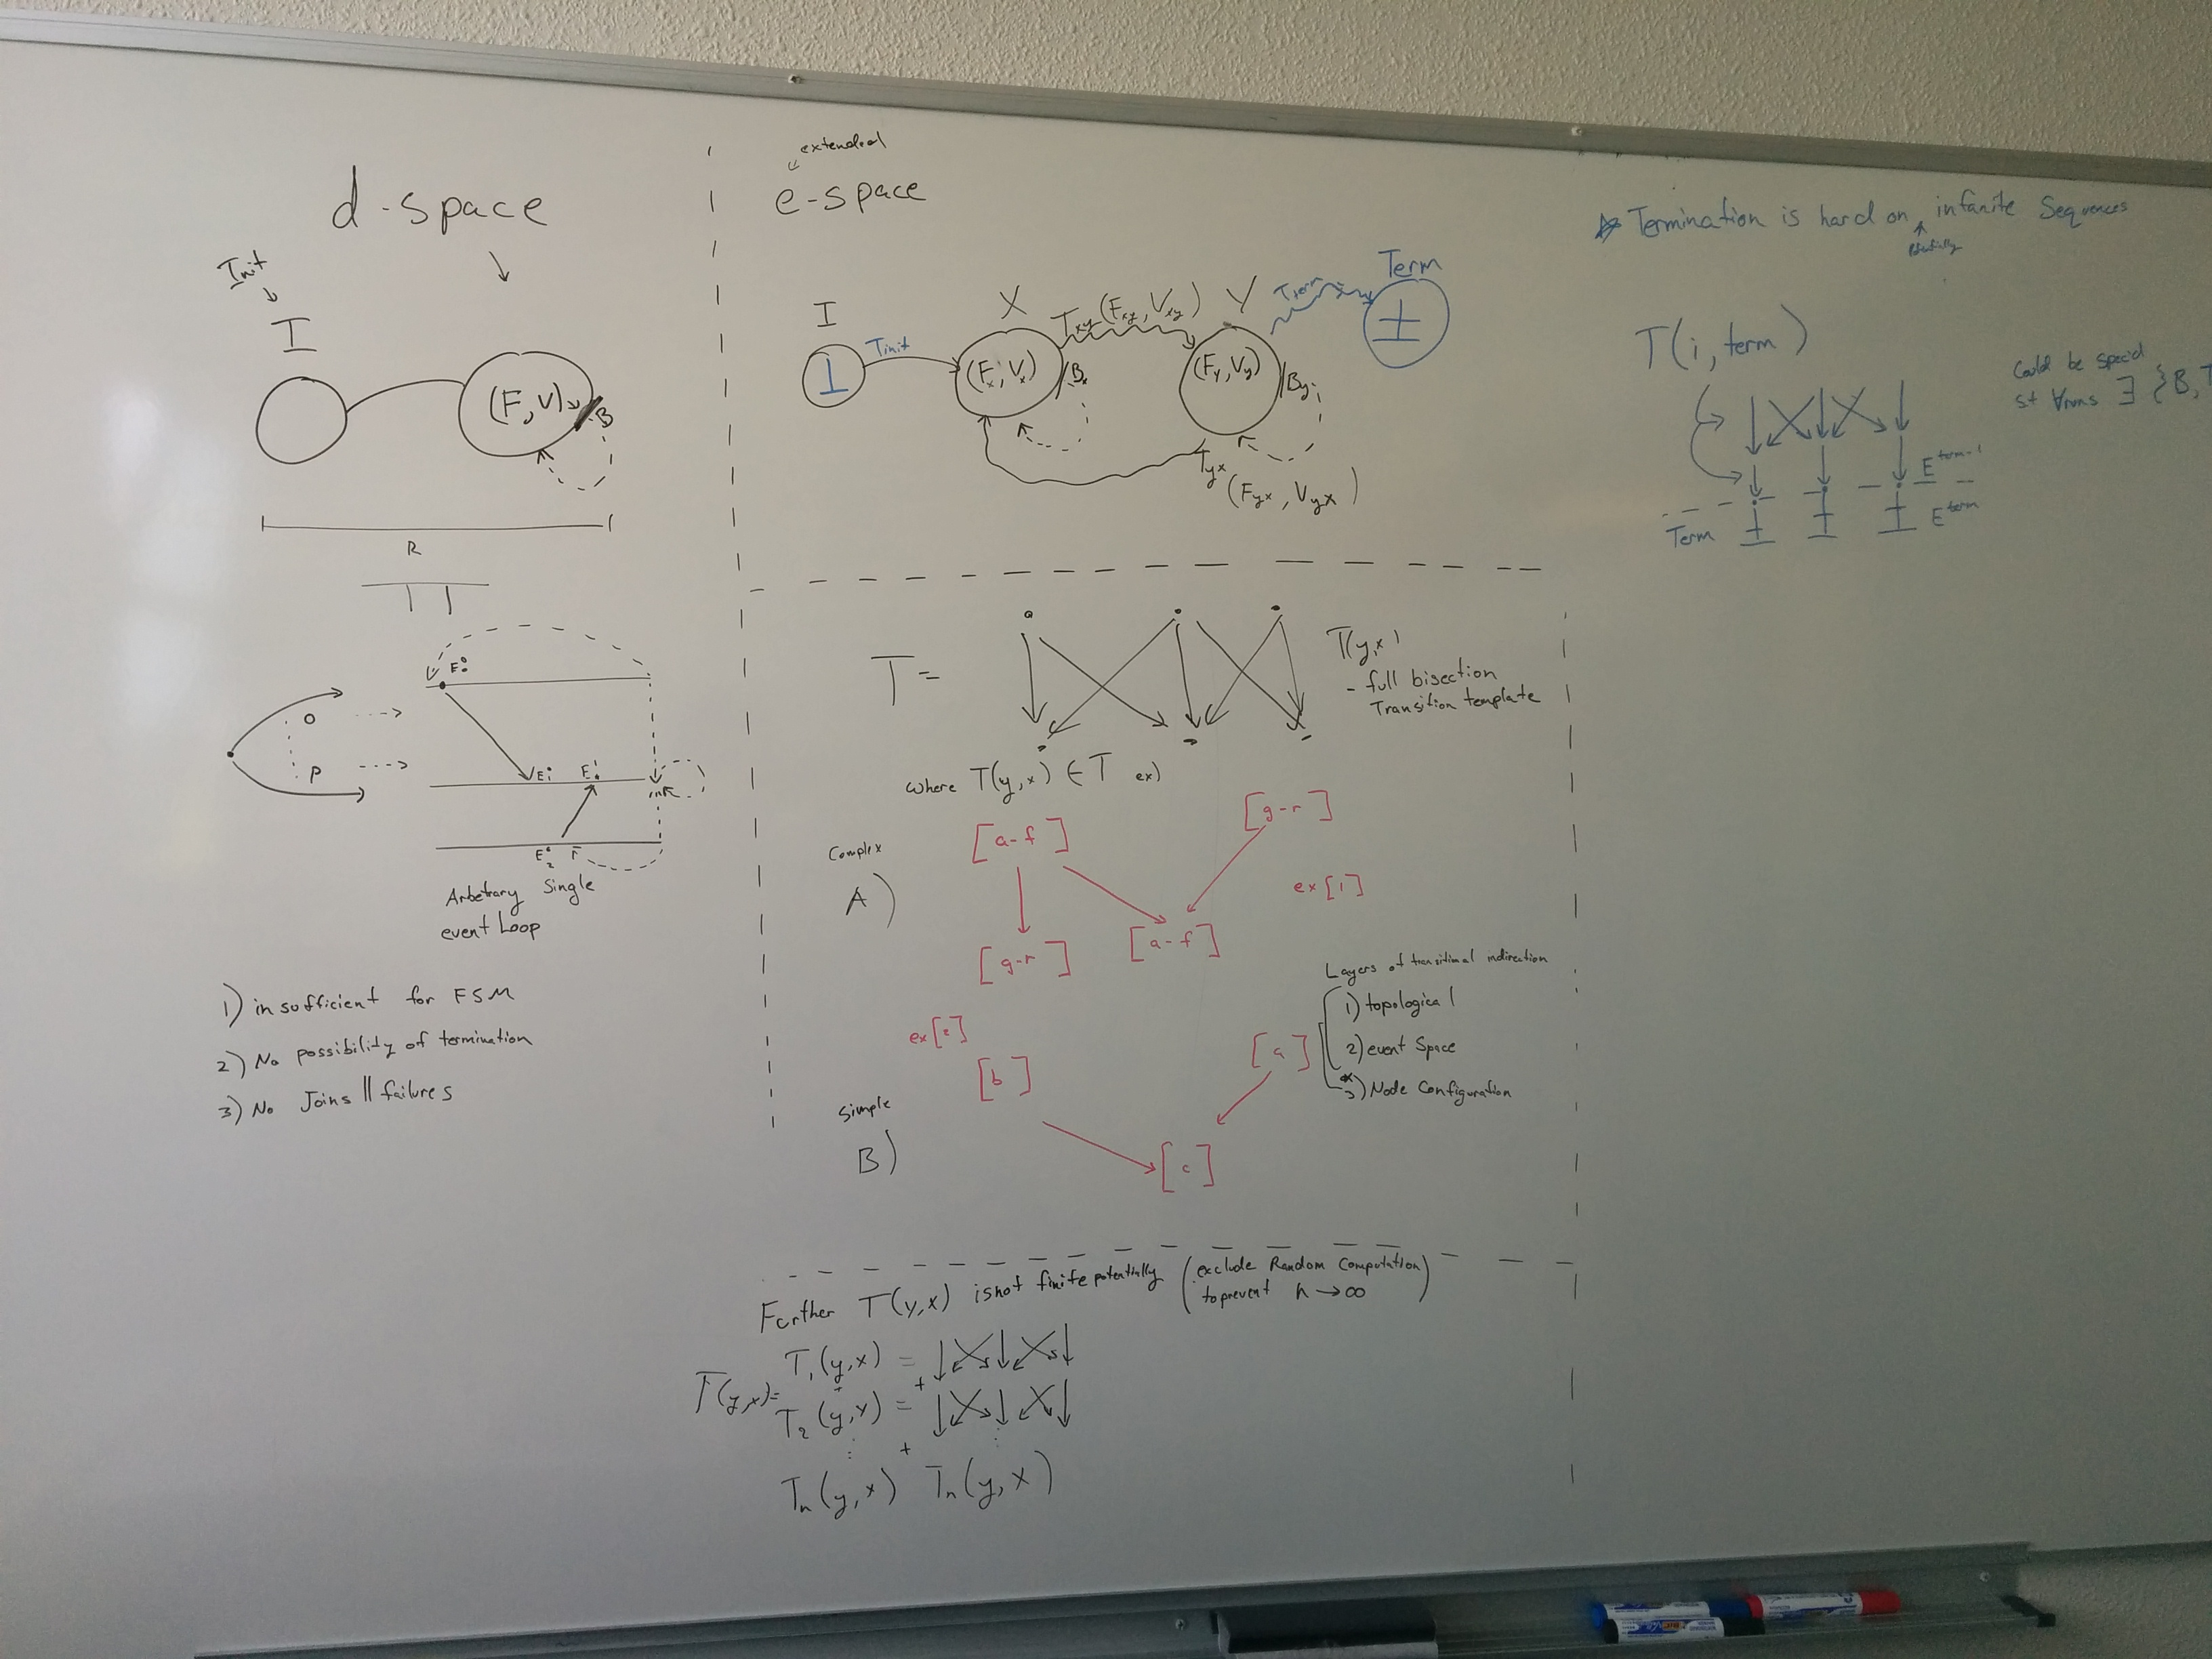
\includegraphics[width=0.50\textwidth]{fig/espace}

    \caption{Sketch of a potential extension to the d-diagram model}

\label{fig:espace} 
\end{figure}


\begin{itemize}

\item{addition of new nodes}

\item{failure of a node}

\item{loss of messages \textit{I think?}}

\item{non deterministic accesses}

\item{Recovery / Fault detection / Reconfiguration}

\end{itemize}

I believe that a more complete model would generalize \textit{d-diagrams} to be
similar to lego blocks, or components of a generalized state machine of a
computation (but I'll finish the paper before jumping on this).



\section{AutoSynch: An Automatic-Signal Monitor Based on Predicate tagging \\ 
\small{Wei-Lun Hung, Vigay K. Garag}}

\subsection{notes}

This paper aims to automate signaling around thread access to shared objects in
Java. The key idea is that signaling requires expertise and a lot of code, but
it is really the same code each time. The authors build a library Autosynch,
which signals waiting threads when predicates become true automaticly,
eliminating the need for thread specific signaling, and reducing the number of
blunt calls to \emph{SignalAll()}.

The meat of this paper, and a lot of the key insights seem to come from the
evaluation of local predicates. The key challange is that from the perspective
of a global moniter, local variables are invisable. Evaluating predicates composed of only global variables is trivial (according to the paper).

The authors make an interesting observation, about the performance of checking
predicates on the fly. They tag predicates in order to check them when values
change. Where some predicate $P = c_0 \wedge c_1 \wedge \dots \wedge c_n$. They
only tage the first conjunction $c_0$. The reasoning behind this is that all
conjunctions needto be true, so whenever any of them change it would be a good
reason to evaluate the predicate, except that it causes overhead. The idea is
check only when a single predicate changes, and hope that the rest are too. It
reduces the checking overhead by a lot I imagine.

They use an interesting heap structure to optimize signaling and checking.
Essentially they order threashold tags into a heap of equivilance ie $x < 5$ is
checked before $x < 7$ for unsigned ints because the space is smaller.
Aparantly this improves the speed of search. If I want to implement something
like this the heap may be key to getting good performance.

After working through the eval it seems clear that the real benifit to this
work is the simplicity of code, while still retaining performance. In most
cases they have to drive the number of threads up into the hundreds before they
see a performance win.

\subsection{observations}

Local predicates can be evaluated by treating their runtime values as constant.
The moment that the \textit{AutoSynch.WaitUntill($P$)} is executed and $P$
contains some local variables $L$ all variables $v \in L$ have their values
logged so the predicate can be evaluated globally.

The key insight to this paper is really that given a set of predicates, the
problem of issuing a signal to a waiting thread is as simple as finding a
waiting thread, not issuing signals to all. This approach requires a
centralized approach to issuing locks.


\begin{figure}[t]
    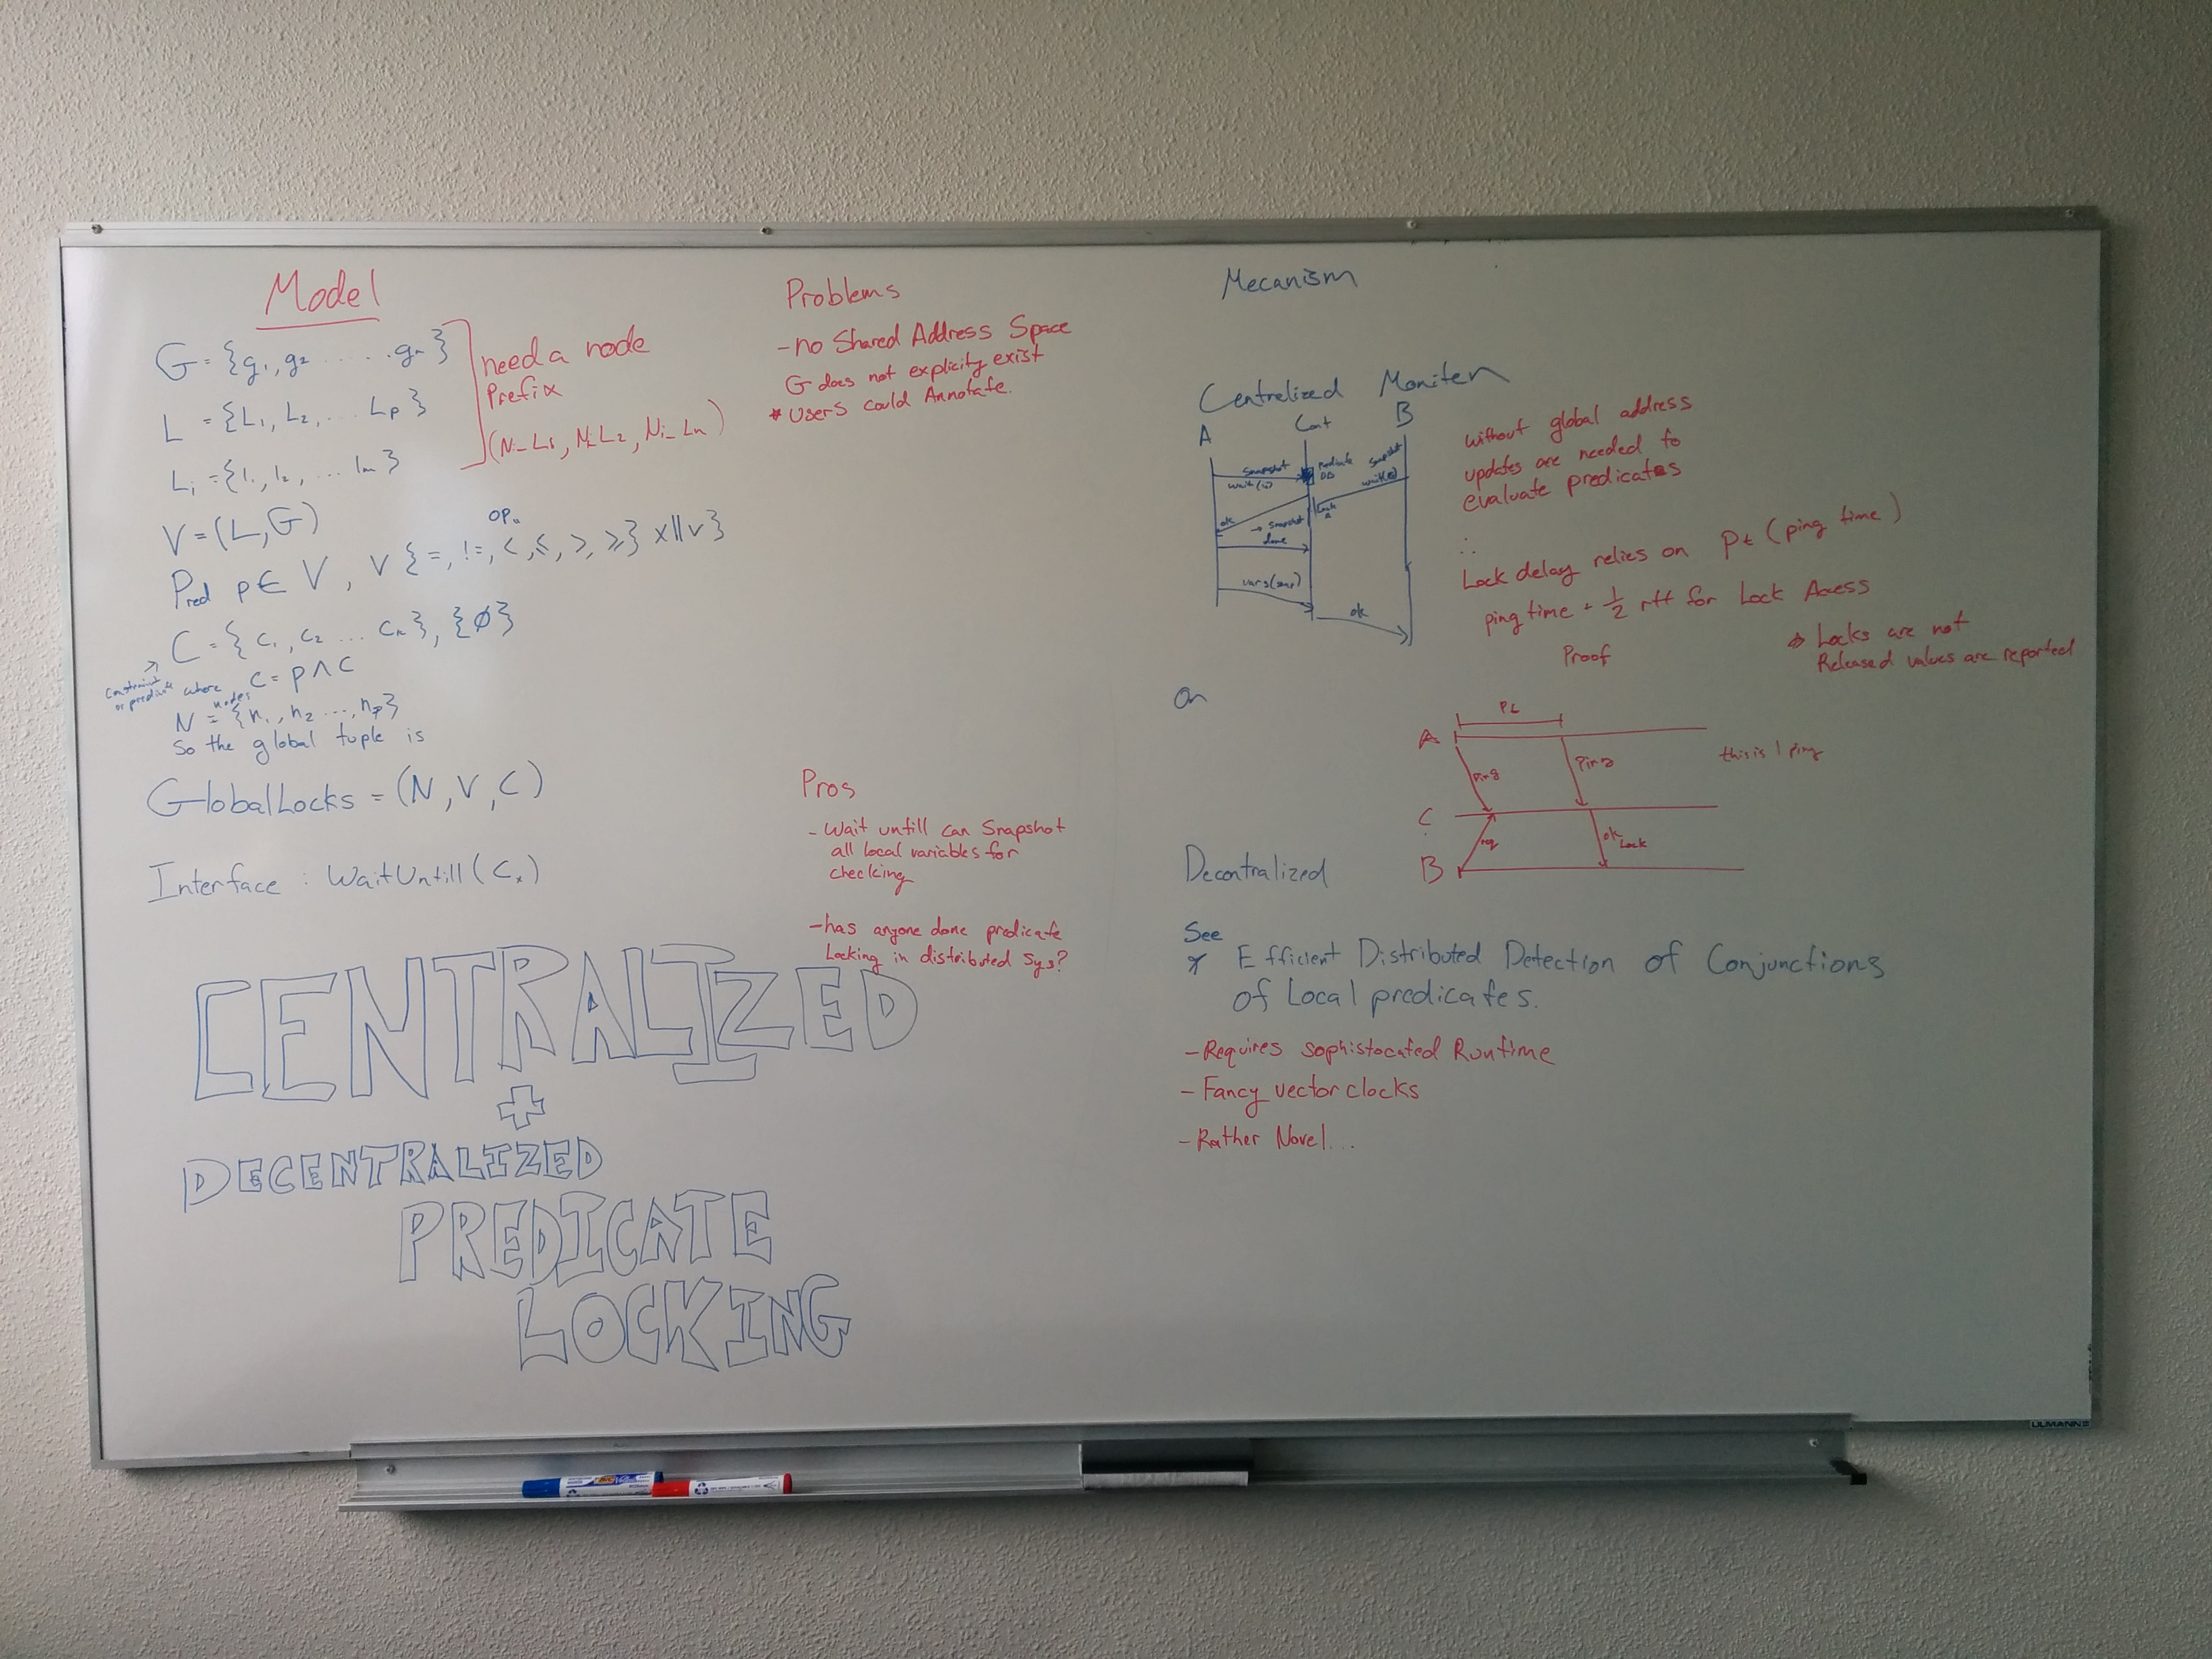
\includegraphics[width=0.50\textwidth]{fig/predicatelock}

    \caption{Whiteboard of potential distributed (centralized and
    decentralized) predicate locking}

\label{fig:espace} 
\end{figure}

\subsection{questions}

\begin{itemize}

    \item How do decentralized lock servers deal with fine grained locking such
as this. In the case of chubby the expection was that locks would last a long
time~\cite{Burrows:2006:CLS:1298455.1298487}. Has work been done where only
waiting threads are issued signals based on predicate evaluation, and not just
locks?

    \item Can the evaluation of predicated be done without a centralized source, and in an online fashion?

\end{itemize}



\section{Deadlocks in Datacenter Networks: Why Do They Form, and How to Avoid Them \\ \small{Shuihai Hu, Yibo Zhu, Peng Cheng, Chuanxiong Guo, Kun Tan, Jitendra Padhye, Kai Chen}}

\subsection{notes}

From the intro and problem definition this paper is of little interest to me.
The authors state that there should be more research into the feild of
deadlocks in networks with lossless messages.

Their reson is that RoCE requires lossless communication channels, these
channels use pauses to mittigate traffic and prevent overflow. If there is a
cycle a deadlock can occur. They cite ~\cite{rdma-commodity-ethernet-scale},
from andys class, where deadlocks occured because of some gap in ARP updates.

While this is true you really have to buy into RDMA, and believe that lossless
channels are a real thing.

The key takeaway here is the formula $r > r_d = \frac{nB}{TTL}$ which
essentially sates that if the incomming amount of data is larger than what is
being taken out the system will deadlock. It ties into the idea that rd is
mittigated by the $TTL$ of any given packet.

\subsection{observations}

The problem of FIFO lossess channel deadlock has not been solved aperently.
After a cursory reading this may acually be a use case for smarter routers.
Potentially ones that could implement RoCE lossless protocols and pass markers
along channes as part of a header to prevent deadlocks.

\subsection{questions}

\begin{itemize}

\item Is this deadlock formulation a real problem? The calculation I would like
to see is how often do these CBD occur, and when they do, how long does it take
to reset? If that number is higher then the overhead introduced by any sort of
deadlock detection algorithm, then the algorithm is unnessisary in a production
enviornment.

\item Are any of these observations corrorborated by datacenters? They only
supply one reference

\item What would the overhead be of using a smart switch to detect deadlocks?
Would it nullify the boost of RDMA?

\end{itemize}

\section{Disks for Data Centers \\ \small{Eric Brewer, Lawrence Ying, Lawrence
Greenfield, Robert Cypher, Theodore Ts'o}}

\subsection{notes}

This has nothing to do with anything really but it probably has some roots with
dataflow problems, and keeping data moving, so I'm going to read it.

The authors point out that disks for data centers do not require the same low
error rate that comodidy PC's require. This is due to the fact that all data
center data is nessisarily replicated globally. Reconstructing damaged data is
easy, so faster disks with higher capacity would be a boon at the loss of
accuracy.

A common practice for disk IO in a data center is to query many disks, and
return the value of the fastest read. Other reads are cancelled. The objective
to try and hit a cache, and gain minimal latency.

An interesting point by the authors is the want to allow disks to opperate
after head failures. They state that they can work around such failures, and it
would increase the lifespan of the disk. This is how you know you are working
at real scale.

\subsection{observations}

The authors of this paper really make one single point. Data centers want finer
grain control over disks. To rationalize this they use the end-to-end principle
as a basis. Essentially they are allready mannaging their own data, and have
very specific use cases for the disk, so many of the optimizations applied by
disk manufactures simply to not apply to them.

As stated above, the future of data center disks may be tall stacked, small
platters with inreliable IO.

Disk API's are a key concern for google practitoners. A potentially interesting
endevor would be to spec out an API for the modern disk, ie rather than flush
commands something like stream(start,finish,rate) would allow for per quality
streaming at a dedicated rate, while allowing for other types of IO to occur
concurently.

Another may be WriteBig(x, size) where a large portion of a disk is written
sequentailly in a part of the disk which can be sequentally read.

\subsection{questions}

\begin{itemize}

\item Are the projections of this paper true? Will disks remain relvent for the
next decade or will Flash take over. If disks are relevent, then for how long?

\item Do these companies actually know what they want? Dispite the apperant
knowledge of disks (at least to the point of their weak points and performance,
are companies such as Google, Facebook, and Amazon really ready to build all of
their systems for custom disks? The extra control may prove to cause larger
errors then they are ready for.

\end{itemize}

\section{Incremental, Iterative Data Processing with Timely Dataflow \\ \small{ P Derek G. Murray, Frank McSherry, Micheal Isard, Rebecca Isaacs, Paul Barham, Martin Abadi}}

\subsection{notes}

This is a simplified version of the Naiad paper, but it is for public
consumption so perhaps it will be a good read none the less. It will also be
good to catch up on Naiad.

This paper was a bit of a waste of time to read, as it covered the details of
Naiad in less detail than the original paper.

Timely data flow is the key contribution to this work, although it was allready
presented in Naiad. The Idea is that distributed dataflow can be modeled as a
dataflow graph and itterations are possible by timestamping events, and using
partial ordering to determine if events are ready for processing.

One key advantage of Naiad is that it does not rely on the \textit{"think like
a vertex"} model of distributed computing. More robust algorithms are possible,
but are more complicated to implement than in a framework such as Pregal.

\subsection{observations}

\subsection{questions}

\begin{itemize}

\item Is Naiad the be all end all, what is needed to make distributed dataflow
more expresive? Is that extra expressiveness nessisary?

\item How bad is scheduling in Naiad in the worst case? Where does this
framework perform poorly.


\end{itemize}





\section{Design patterns for container-based distributed systems \\ \small{Brendan Burns, David Oppenhimer}}

\subsection{notes}

The first substantial claim of this paper is that containers are essentiall the
object's of distributed computing. My instinct is to disagree because they all
take the same form and are shaped from the inside rather than the outside. For
instance it is expensive and uncommon to wrap a container in another container.
But perhaps that is a short sighted statement.

The authors aruge that contains should be embued with a similar API to Android
Apps, ie \textit{run(), pause(), stop()} are insufficient, and additional
callback functions such as \textit{onCreate(), onStart(), onStop()} would be
usefull.

As a whole I do not really agree with the sentement of this work. Containers
are simply not the same as objects as they do not conform, nor could they
easily conform to the heirarcies which are applied to objects and which make
them powerful, such as inheritance, encapulation and polymorphism. 

What they present here is work partitioning. They treat containers as libraries
not as objects, which I do agree with. What this paper should acknowledge is
that Containers are like library code which has a front facing api.

In most of there examples they simply put a container in between two pieces of
existing infrastructure to isolate the developemnt of custom software.

\subsection{observations}

At it's core, it seems correct that containers should be used as building
blocks for systems, at least for the sake of simplicity. What is not mentioned
here is performance, which is clearly not a concern of the authors

What would be interesting in my opinion would be a flexable container where
oversubscription is delt with automatically and configurations change on the
fly to meet with demand. It would be very interesting to see if an ecosystem
such as naiad would allow for dynamic allocation of new resources on the fly.

The key patterns here are \textit{sidecar}: a app that works off  to the side
to perform background tasks, like backups or analytics. \textit{ambassador /
proxy} a container that sits between an app and the real network.
\textit{interface}: Sits between a legacy system and a new app. \textit{Work
queue}: By far the most interesting, here we have complicated tasks like leader
election, being taken over by a containerized solution.


\subsection{questions}

\begin{itemize}

\item Are there techniques for automatically scaling the deployment of
containerized applications? (Yes there are for example \textit{Elastic stateful Stream processing in Storm}

\item What is the overhead of using these patterns? Is there a significant
slowdown by placing an interface between one system and another.

\end{itemize}

\section{Encoding, Fast and Slow: Low-Latency Video Processing Using Thousands of Tiny Threads \\ \small{sadjad Fouladi, Riad S. Wahby, Brennadn Shacklett, Karthikeyan Vasuki Balasubaramaniam, William Zeng, Rahul Bhalero, Anirudh Sivaraman, George Porter, Keith Winstein}}

\subsection{notes}

\subsection{observation}

\subsection{questions}

\begin{itemize}

\end{itemize}


\balance
\bibliographystyle{abbrv}
\bibliography{paper}

\end{document}
